\begin{Chapter}

\chapter{Title Example 2}

\section{Section Header Level 1}

Content Text Content Text Content Text Content Text Content Text Content Text Content \cite{knuth:1984} Text Content Text Content Text Content Text Content Text Content Text Content Text \cite{latex2e}, Content Text Content Text Content Text Content Text Content Text Content Text Content Text Content Text Content Text Content Text Content Text Content Text Content Text.

\begin{table*}[htbp]
    \centering
    \caption{Another table caption} \label{tab: complexity}
    \makebox[\linewidth][c]{
    \renewcommand\arraystretch{1.2}{
        \begin{tabular}{| l | c  c  c  c |}
        \hline
        Protocol & $P$ & $CS_1$ & $CS_2$ & $RG$ \\
        \hline
        MSSMul & $O(1)$, $O(1)$, N/A & $O(n-t)$, $O(n)$, $O(1)$ & $O(n-t)$, $O(n)$, N/A & $O(1)$, $O(n)$, $O(n)$ \\
        SC & $O(1)$, $O(1)$, N/A & $O(n-t)$, $O(n)$, $O(1)$ & $O(n-t)$, $O(n)$, N/A & $O(1)$, $O(n)$, $O(n)$ \\
        \hline 
        \end {tabular}
    }}
\end {table*}

\section{Section Header Level 1}

Content Text Content Text Content Text Content Text Content Text Content Text Content Text Content Text Content Text Content Text Content Text Content Text Content Text.

\begin{figure*}[htbp]
    \centering
    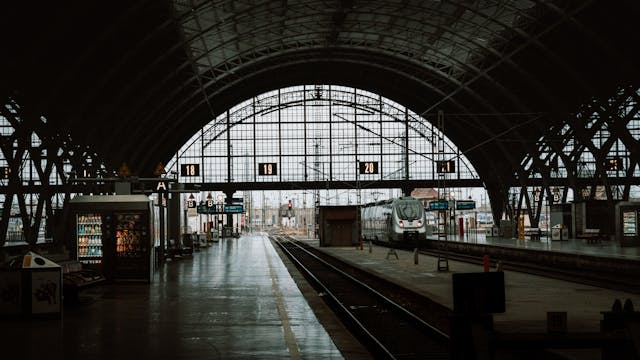
\includegraphics[width = 0.5\textwidth]{pics/image.jpeg}
    \caption{Cool train station}
    \label{fig: image}
\end{figure*}

\begin{figure}[ht]
    \centering
    \begin{minipage}{\linewidth}
        \centering
        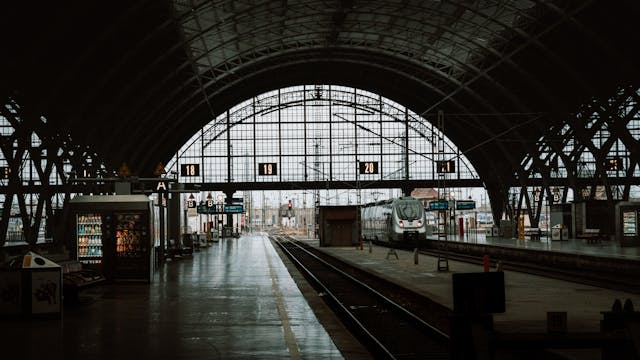
\includegraphics[width=\linewidth]{pics/image.jpeg}
        \vspace{0.5ex}
        \small (a)
    \end{minipage}
    \vspace{0.5em}
    
    \begin{minipage}{\linewidth}
        \centering
        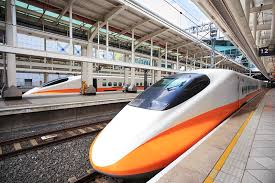
\includegraphics[width=\linewidth]{pics/train-station2.jpeg}
        \vspace{0.5ex}
        \small (b)
    \end{minipage}
    \caption{Illustration of the train stations: (a) and (b) (Continued in Figure~\ref{fig2-cont})}
    \label{fig2}
\end{figure}

\begin{figure}[ht]
    \centering
    \begin{minipage}{\linewidth}
        \centering
        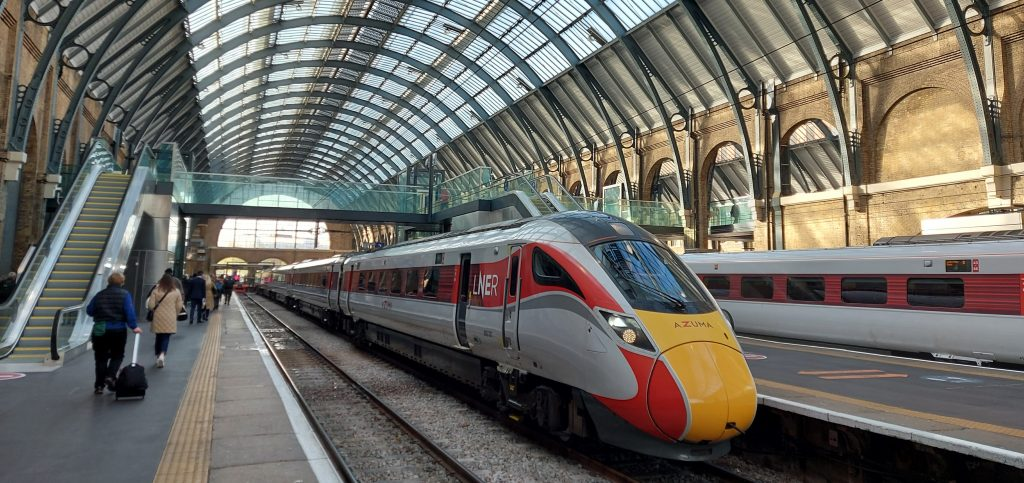
\includegraphics[width=\linewidth]{pics/train-station3.jpg}
        \vspace{0.5ex}
        \small (c)
    \end{minipage}
    \vspace{0.5em}
    
    \begin{minipage}{\linewidth}
        \centering
        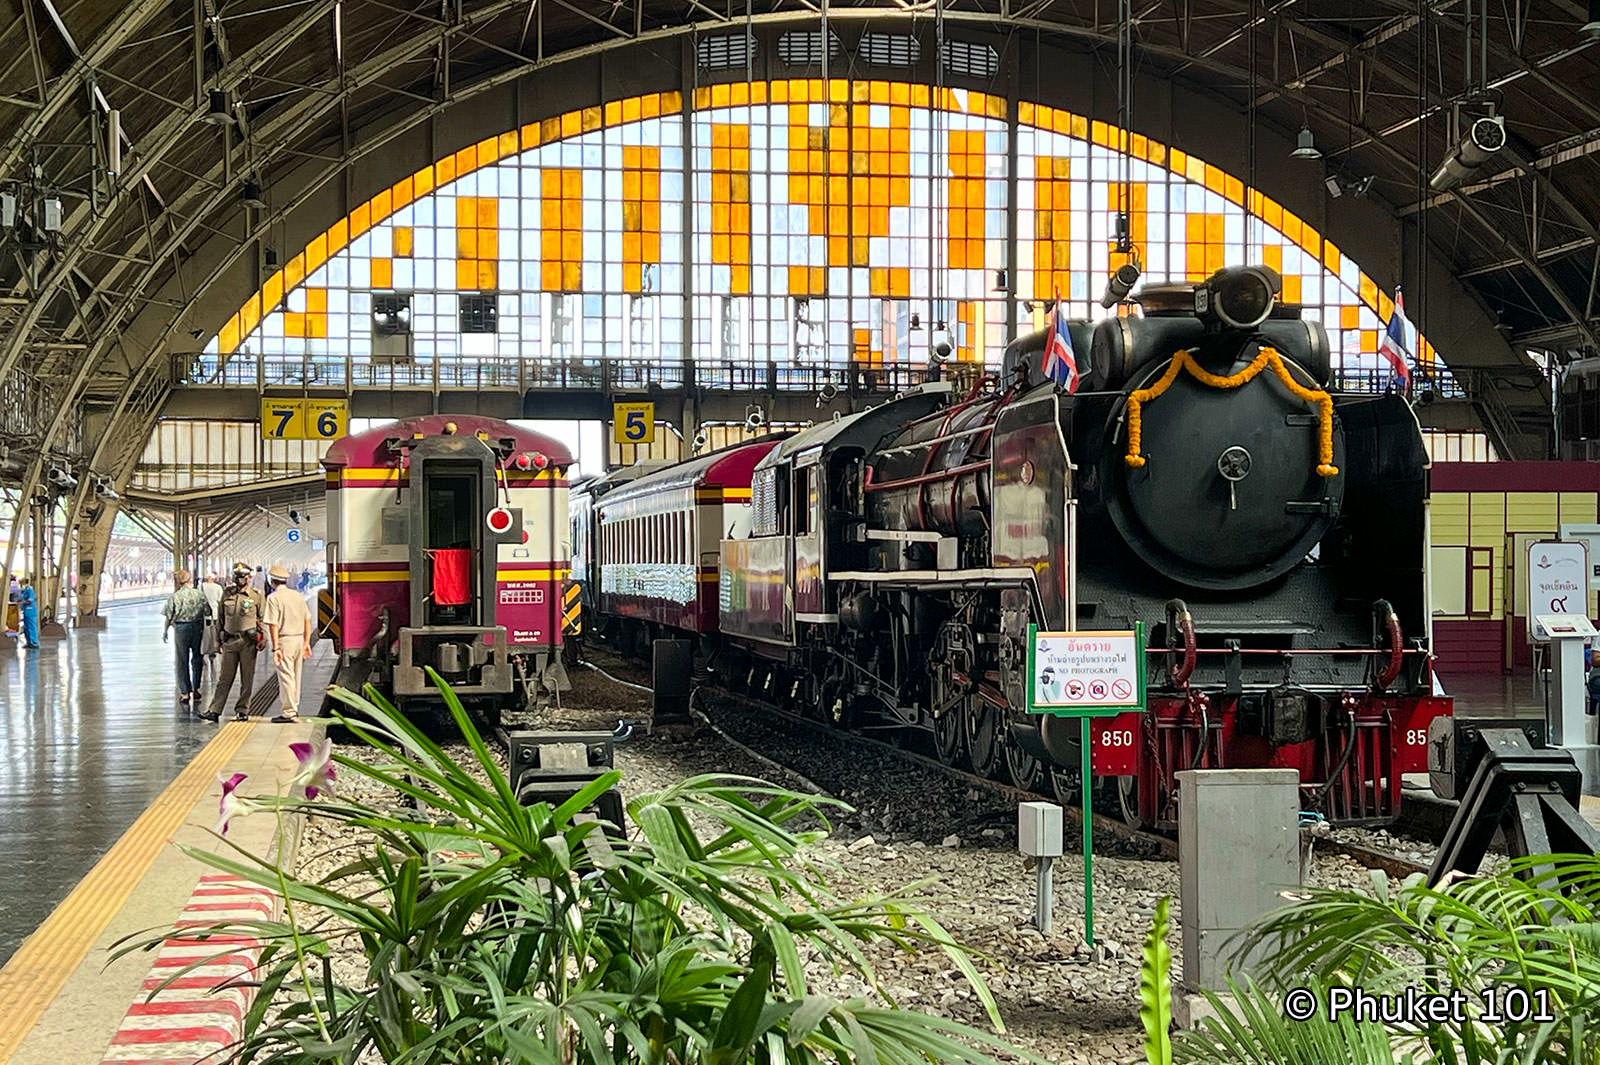
\includegraphics[width=\linewidth]{pics/train-station4.jpg}
        \vspace{0.5ex}
        \small (d)
    \end{minipage}
    \caption{Illustration of the train stations: (c) and (d)}
    \label{fig2-cont}
\end{figure}

You may also, somehow, need to put a very looong table into your work, which is fine, and I understand. You could put it like the table \ref{sec.longtable}

\begin{longtable}{|p{0.3\textwidth}|p{0.25\textwidth}|p{0.35\textwidth}|}
\caption{A very loooong table} \label{sec.longtable}\\
\hline
\textbf{Category}& \textbf{ID}& \multicolumn{1}{|c|}{\textbf{Comment}} \\
\hline
\endfirsthead

\hline
\multicolumn{3}{|c|}{Continuation of Table \ref{sec.longtable}}\\
\hline
\textbf{Category}& \textbf{ID}& \multicolumn{1}{|c|}{\textbf{Comment}} \\
\hline
\endhead

\hline
\endfoot

\hline
\multicolumn{3}{|c|}{End of Table \ref{sec.longtable}}\\\hline
\endlastfoot

\textbf{1\_Foo}& \textbf{Bar}& 0\_Foo \\
&&1\_Bar\\
&&2\_Foo\\
&&3\_Bar\\
&&4\_Foo\\
&&5\_Bar\\
&&6\_Foo\\
&&7\_Bar\\
&&8\_Foo\\
&&9\_Bar\\
&&10\_Foo\\
&&11\_Bar\\
\hline
\textbf{2\_Foo}& \textbf{Bar}&12\_Foo\\
&&13\_Bar\\
&&14\_Foo\\
&&15\_Bar\\
&&16\_Foo\\
&&17\_Bar\\
&&18\_Foo\\
&&19\_Bar\\
&&20\_Foo\\
&&21\_Bar\\
&&22\_Foo\\
&&23\_Bar\\
&&24\_Foo\\
&&25\_Bar\\
&&26\_Foo\\
&&27\_Bar\\
&&28\_Foo\\
&&29\_Bar\\
&&30\_Foo\\
&&31\_Bar\\
&&32\_Foo\\
&&33\_Bar\\
&&34\_Foo\\
&&35\_Bar\\
&&36\_Foo\\
&&37\_Bar\\
&&38\_Foo\\
&&39\_Bar\\
&&40\_Foo\\
&&41\_Bar\\
&&42\_Foo\\
&&43\_Bar\\
&&44\_Foo\\
&&45\_Bar\\
&&46\_Foo\\
&&47\_Bar\\
&&48\_Foo\\
\hline
\textbf{3\_Foo}&\textbf{Bar}&49\_Bar\\
&&50\_Foo\\
&&51\_Bar\\
&&52\_Foo\\
&&53\_Bar\\
&&54\_Foo\\
&&55\_Bar\\
&&56\_Foo\\
&&57\_Bar\\
&&58\_Foo\\
&&59\_Bar\\
\hline
\end{longtable}

\end{Chapter}